\documentclass[conference]{IEEEtran}

% ------------------------------------------------
% Packages
% ------------------------------------------------
\usepackage{amsmath, amssymb}
\usepackage{graphicx}
\usepackage{cite}
\usepackage{url}
\usepackage{xurl}
\usepackage{booktabs}
\usepackage{array}
\usepackage{float}
\usepackage{algorithm}
\usepackage{algpseudocode}
\usepackage{balance}       % iguala las dos columnas de la última página
\renewcommand{\refname}{Bibliografía}
\renewcommand{\tablename}{Tabla}
\renewcommand{\abstractname}{Resumen}
\floatname{algorithm}{Algoritmo}
\algrenewcommand\algorithmicrequire{\textbf{Entrada:}}
\algrenewcommand\algorithmicensure{\textbf{Salida:}}
% Todas las figuras y cifras salen del código del repositorio (scripts/)
\graphicspath{{../../outputs/figuras/}}
% ------------------------------------------------
% Document
% ------------------------------------------------
\begin{document}

% ------------------------------------------------
% Title
% ------------------------------------------------
\title{Evaluación de la Vulnerabilidad de la Red Vial Primaria de Carga de Colombia Mediante Teoría de Grafos}

% ------------------------------------------------
% Authors
% ------------------------------------------------
\author{
    \IEEEauthorblockN{
        David Catral,
        Gabriel Salcedo,
        Isaac Suárez
    }
    \IEEEauthorblockA{
        Escuela de Economía y Negocios\\
        Universidad del Rosario\\
        Bogotá, Colombia\\
\{jose.catral, gabriel.salcedo, isaac.suarez\}@urosario.edu.co    }
}

\maketitle

\begin{abstract}
Se modela la red vial primaria de Colombia como un grafo ponderado por el costo
de mover una tonelada (53 vértices y 77 aristas construidos a partir de la capa
de INVIAS) y se le asigna la carga del RNDC de 2015 entre las 25 ciudades con
más carga. Con Dijkstra, Brandes y Tarjan se mide, para cada tramo, su posición
en la red, la carga que lo atraviesa y el daño que produce su cierre: el
sobrecosto anual de la carga que se desvía y las toneladas que se quedan sin
ruta. La red es frágil ($\kappa=\lambda=1$, tres puentes): cerrar
Buenaventura--Dagua deja sin ruta 9,45 millones de toneladas al año, y cerrar
Buga--Zarzal cuesta 908,6 mil millones de pesos al año. Las tres medidas están
correlacionadas, pero solo dos aristas aparecen a la vez entre las diez primeras
de las tres: mirar solo la posición en el mapa sobrestima unos corredores y
subestima otros. El código, los datos y una herramienta interactiva de rutas
y cierres son públicos y reproducibles.
\end{abstract}


% ------------------------------------------------
% I. Introducción
% ------------------------------------------------
\section{Introducción}
Una red de transporte se representa de forma natural como un
grafo ponderado: los vértices son localidades o cruces, las aristas son los
tramos viales que los conectan y el peso de cada arista es el costo de
recorrerla. Sobre esa representación, la teoría de grafos ofrece herramientas
directas para estudiarla. El algoritmo de Dijkstra \cite{dijkstra1959} calcula
la ruta de mínimo costo entre dos puntos; la centralidad de intermediación
\cite{brandes2001} mide qué componentes concentran el tránsito de la red; y la
búsqueda en profundidad \cite{tarjan1972} identifica los puentes, es decir, las
aristas cuya remoción desconecta el grafo.

En Colombia estas herramientas tienen una aplicación inmediata. La geografía
montañosa y la distancia entre los centros de producción, los puertos y los
principales mercados hacen que el transporte de carga dependa de un número
reducido de corredores troncales y transversales, que conforman la red vial
primaria \cite{ocha_hdx_roads}. Cuando uno de esos tramos se cierra por
derrumbes, crecientes, bloqueos u obras, la carga debe tomar una ruta alterna
más larga y más costosa, y en algunos casos no existe ruta alterna
\cite{cambio_radiografia}. Saber de antemano cuáles tramos producen el mayor
daño permitiría priorizar el mantenimiento y la inversión sobre criterios
objetivos.

Este proyecto modela la red vial primaria como un grafo ponderado, le asigna los
flujos de carga reportados en el Registro Nacional de Despachos de Carga por
Carretera (RNDC) \cite{rndc}, identifica los tramos críticos y estima el
sobrecosto de las rutas alternas que resultarían de su cierre. El enfoque sigue
la línea de trabajo sobre vulnerabilidad de redes viales, que mide la
importancia de un tramo por el aumento de costo que produce su interrupción
\cite{jenelius2006}. El resto del documento está organizado de la siguiente
manera. La Sección~\ref{sec:descripcion} describe el problema y la
Sección~\ref{sec:objetivos} presenta los objetivos. La
Sección~\ref{sec:marco} explica los conceptos en los que se apoya el
análisis, la Sección~\ref{sec:modelo} describe cómo se construyó el
modelo y la Sección~\ref{sec:solucion} presenta la solución propuesta. La
Sección~\ref{sec:implementacion} describe su implementación, la
Sección~\ref{sec:resultados} presenta los resultados y la
Sección~\ref{sec:conclusiones} las conclusiones.

% ------------------------------------------------
% II. Descripción del Problema
% ------------------------------------------------
\section{Descripción del Problema}
\label{sec:descripcion}

% PENDIENTE (decisión del equipo): 85,7 millones de t es la carga reportada solo en
% kilos; la matriz O-D que usa el modelo suma 93,0 millones. Ver AUDITORIA.md §5.2.
El transporte por carretera moviliza la mayor parte de la carga interna del
país. Solo en el año 2015, el RNDC registra cerca de $6$ millones de viajes y
$85{,}7$ millones de toneladas despachadas entre municipios \cite{rndc}. Toda
esa carga circula sobre una red primaria que sufre cierres frecuentes por
eventos naturales, bloqueos y obras de mantenimiento \cite{cambio_radiografia}.
Cada cierre obliga a desviar los vehículos por rutas más largas, lo que aumenta
la distancia recorrida, el tiempo de viaje y el flete pagado, y ese sobrecosto
termina reflejándose en el precio final de los bienes transportados.

El problema es que no resulta evidente cuáles tramos son realmente críticos. Un
tramo puede ocupar una posición central en la red y sin embargo transportar poca
carga, porque la demanda de transporte no se reparte de manera uniforme sobre el
territorio. Otro puede mover un volumen alto y tener una vía paralela de costo
similar, de modo que su cierre casi no afecta al sistema. Lo que hace crítico a
un tramo es la combinación de dos cosas: cuánta carga lo utiliza y qué tan buena
es su mejor alternativa. Responder esa pregunta exige un modelo que integre la
estructura física de la red con el uso real que se hace de ella, y la teoría de
grafos permite construirlo de forma cuantitativa y reproducible, en lugar de
depender de percepciones sobre cuáles vías son importantes.

% ------------------------------------------------
% III. Objetivos (General y Específicos)
% ------------------------------------------------
\section{Objetivo General y Objetivos Específicos}
\label{sec:objetivos}
\subsection{Objetivo General}
Evaluar la vulnerabilidad de la red vial primaria de carga de Colombia mediante
teoría de grafos, identificando sus tramos críticos y cuantificando el
sobrecosto de transporte de las rutas alternas que resultarían de su
interrupción.

\subsection{Objetivos Específicos}
\begin{itemize}
    \item Construir la red vial primaria nacional como un grafo ponderado a
    partir de la capa vial de INVIAS publicada por OCHA Colombia en la
    plataforma HDX \cite{ocha_hdx_roads} y caracterizar su estructura:
    orden, tamaño, componentes conexas, puentes y vértices de corte.

    \item Construir la matriz origen--destino de carga a partir del RNDC y
    asignarla sobre el grafo mediante rutas de costo mínimo, validando las
    distancias estimadas contra los kilómetros reportados en los despachos.

    \item Identificar los tramos críticos de la red contrastando su
    centralidad topológica con la carga que efectivamente los atraviesa.

    \item Simular el cierre de dichos tramos y cuantificar el sobrecosto de
    transporte de la ruta alterna, así como el volumen de carga que quedaría sin
    ruta disponible.
\end{itemize}

% ------------------------------------------------
% IV. Marco Teórico
% ------------------------------------------------
\section{Marco Teórico}
\label{sec:marco}

Los conceptos básicos de la teoría de grafos, como grafo ponderado, camino,
conexidad, componente conexa, puente y vértice de corte, y algoritmo de Dijkstra, se dan por conocidos
\cite{diestel2017}. Esta sección explica los conceptos que el proyecto añade
sobre esa base, en el mismo orden en que se usan: primero cómo se mide el costo
de transportar carga y cómo se representa la demanda, después cómo se reparte
esa demanda sobre la red, luego cómo se mide la importancia de un tramo y por
último cómo se mide el daño que produce su cierre.

\subsection{Costo de transporte y ruta más barata}
\label{sub:costo}

En la mayoría de aplicaciones de rutas el peso de una arista es su longitud. En
transporte de carga, sin embargo, lo que decide la ruta de un transportador es
el costo de recorrerla, que incluye la operación del vehículo, el tiempo y los
peajes; la literatura de transporte lo llama \emph{costo generalizado}
\cite{ortuzar2011}. En este proyecto ese costo se aproxima con el \emph{flete}:
lo que efectivamente se paga por mover una tonelada un kilómetro, en pesos por
tonelada--kilómetro (COP/t-km). Así, el peso $w_e$ de una arista $e$ es el
costo de mover una tonelada por ella.

Con esos pesos, la ruta más barata $R_{od}$ entre un origen $o$ y un destino
$d$ se obtiene con el algoritmo de Dijkstra \cite{dijkstra1959}, y su costo es
\begin{equation}\label{eq:cmin}
c_G(o,d)=\sum_{e\in R_{od}} w_e .
\end{equation}
Si no existe ningún camino entre $o$ y $d$, se escribe $c_G(o,d)=\infty$. Esta
cantidad es la base de todo lo que sigue: tanto la importancia de un tramo como
el daño de su cierre se miden comparando costos mínimos.

\subsection{Matriz origen--destino}
\label{sub:od}

El grafo describe por dónde \emph{se puede} viajar, pero no cuánta carga
\emph{necesita} viajar. Esa información se organiza en la \emph{matriz
origen--destino} $T=[T_{od}]$ \cite{ortuzar2011}: cada fila es un origen, cada
columna un destino, y la entrada $T_{od}$ son las toneladas despachadas de $o$
a $d$ en un año. Por ejemplo, $T_{\text{Bogotá},\,\text{Barranquilla}}$ son las
toneladas que salieron de Bogotá hacia Barranquilla. La matriz no es simétrica:
lo que va de $o$ a $d$ no tiene por qué ser igual a lo que regresa.

La matriz es lo que convierte el análisis de la red en un análisis económico.
Sin ella, todas las parejas de ciudades pesan lo mismo y solo se puede hablar
de la forma de la red. Con ella, cada ruta pesa según las toneladas que
realmente la usan, y los resultados se pueden expresar en toneladas y en pesos.
En este proyecto $T$ cumple tres funciones: indica cuánta carga pasa por cada
tramo, pondera la importancia de cada tramo según esa carga y convierte el
desvío causado por un cierre en un sobrecosto en pesos.

\subsection{Asignación todo o nada}
\label{sub:asignacion}

La matriz $T$ dice cuánta carga va de cada origen a cada destino, pero no por
dónde viaja. Para repartirla sobre las aristas se usa la \emph{asignación todo
o nada} \cite{ortuzar2011}: toda la carga de cada pareja viaja por su ruta más
barata $R_{od}$. La carga que atraviesa una arista $e$ es la suma de las
toneladas de todas las parejas cuya ruta la usa:
\begin{equation}\label{eq:flujo}
x_e=\sum_{(o,d)} T_{od}\,\mathbf{1}\{e\in R_{od}\},
\end{equation}
donde $\mathbf{1}\{e\in R_{od}\}$ vale 1 si la ruta de $o$ a $d$ pasa por $e$ y
0 si no.

Este método supone que no hay congestión: una vía no se vuelve más costosa por
la carga que recibe. Es razonable para carga anual entre ciudades, y tiene una
consecuencia que conviene anticipar: al cerrar una vía, la ruta alterna no se
encarece por la carga adicional, así que el sobrecosto calculado será una
estimación \emph{por debajo} del real.

\subsection{Intermediación de aristas}
\label{sub:btw}

La \emph{intermediación} de una arista mide qué tan indispensable es para
conectar la red. Se define como el número de parejas de vértices cuya ruta más
barata pasa por ella \cite{brandes2001}:
\begin{equation}\label{eq:btw}
C_B(e)=\sum_{(s,t)} \mathbf{1}\{e\in R_{st}\}.
\end{equation}
Una arista con intermediación alta es un paso obligado para muchas rutas. Si una
pareja tiene varias rutas igual de baratas, cada una cuenta en proporción.

Calcular \eqref{eq:btw} listando todas las rutas sería muy costoso. El algoritmo
de Brandes \cite{brandes2001} lo evita: desde cada origen ejecuta un Dijkstra,
cuenta cuántas rutas mínimas llegan a cada vértice y luego recorre los vértices
del más lejano al más cercano, acumulando qué fracción de esas rutas pasa por
cada arista. Su costo es $O(nm+n^2\log n)$ para un grafo de $n$ vértices y $m$
aristas.

La definición \eqref{eq:btw} trata a todas las parejas por igual: la pareja
Bogotá--Medellín cuenta lo mismo que una pareja de ciudades que casi no
intercambian carga. Si en lugar de contar cada pareja una vez se le da el peso
de sus toneladas $T_{st}$, la suma resultante es exactamente la carga $x_e$ de
\eqref{eq:flujo}. Es decir, la carga asignada es una intermediación
\emph{ponderada por la demanda}, y $C_B$ es el caso particular en que todas las
parejas pesan lo mismo. Esta relación es la que permite cumplir el objetivo 3:
comparar $C_B$ con $x_e$ muestra qué tramos parecen importantes solo por su
posición en el mapa y cuáles lo son por la carga que realmente los usa.

\subsection{Puentes y algoritmo de Tarjan}
\label{sub:tarjan}

Un puente es una arista cuya eliminación desconecta el grafo. En una red vial,
cerrar un puente no encarece la ruta: la elimina. Por eso es necesario
identificarlos antes de medir sobrecostos.

El algoritmo de Tarjan \cite{tarjan1972} los encuentra todos con un solo
recorrido en profundidad. Durante el recorrido numera cada vértice $v$ en el
orden en que lo visita, $\text{disc}(v)$, y calcula $\text{low}(v)$: el número
más pequeño al que se puede regresar desde $v$ o sus descendientes usando una
arista que no sea del árbol de recorrido. Si desde $v$ no es posible regresar a
su padre $u$ ni a nada anterior, es decir, si
$\text{low}(v)>\text{disc}(u)$, la única conexión de esa parte del grafo con el
resto es la arista $uv$, y por lo tanto es un puente. Con la misma información
se identifican los vértices de corte. El costo es $O(n+m)$.

\subsection{Medidas de daño}
\label{sub:dano}

Para medir el daño de cerrar una arista $e$ se compara el costo mínimo de cada
pareja antes del cierre, $c_G(o,d)$, con el costo después del cierre,
$c_{G-e}(o,d)$, que es el de la mejor ruta alterna. Siguiendo a Jenelius et al.
\cite{jenelius2006}, el daño se resume en dos cantidades. La primera es el
\emph{sobrecosto} que paga la carga que sí encuentra ruta alterna:
\begin{equation}\label{eq:imp}
I(e)=\sum_{(o,d)\,:\,c_{G-e}(o,d)<\infty} T_{od}\,
\big[\,c_{G-e}(o,d)-c_G(o,d)\,\big].
\end{equation}
La segunda es la \emph{demanda insatisfecha}: las toneladas que se quedan sin
ninguna ruta,
\begin{equation}\label{eq:dem}
D(e)=\sum_{(o,d)\,:\,c_{G-e}(o,d)=\infty} T_{od} .
\end{equation}

Las dos se reportan por separado. Si las parejas sin ruta entraran en
\eqref{eq:imp}, el sobrecosto de todo puente sería infinito y no se podrían
comparar entre sí. $I(e)$ se mide en pesos y $D(e)$ en toneladas.


% ------------------------------------------------
% V. Modelamiento del Problema
% ------------------------------------------------
\section{Modelamiento del Problema}
\label{sec:modelo}

\subsection{Datos}
Se usan tres fuentes públicas: la red vial de INVIAS publicada en HDX
\cite{ocha_hdx_roads}, con 652 tramos y 20.011\,km; el RNDC del Ministerio de
Transporte \cite{rndc}, que registra para cada despacho su origen, destino,
toneladas, kilómetros y valor pagado; y la DIVIPOLA del DANE
\cite{dane_divipola}, para ubicar cada municipio.

\subsection{Construcción del modelo}
\begin{enumerate}
    \item \textbf{Limpiar el mapa.} Se eliminaron tramos duplicados y fuera de
    servicio y se unieron los extremos separados por menos de 50\,m, para que
    las vías que se tocan en la realidad también se toquen en el grafo.
    \item \textbf{Elegir las ciudades.} Se tomaron las ciudades que más carga
    mueven y se agruparon las áreas metropolitanas (por ejemplo, Bogotá con
    Soacha, Funza, Mosquera y Cota). Quedaron 25 ciudades.
    \item \textbf{Construir la matriz $T$.} El RNDC se depuró en R y se sumaron
    las toneladas por pareja de municipios (42.547 parejas). Luego cada
    municipio se asignó a su ciudad, y se obtuvo una matriz de $25\times 25$
    con las toneladas anuales entre ciudades. Esas parejas concentran el
    47\,\% de la carga entre municipios del país.
    \item \textbf{Ubicar los cruces.} Se trazaron las rutas más baratas entre
    las ciudades y se marcaron los puntos donde se separan, como La Pintada u
    Honda. Quedaron 28 cruces: son los puntos donde un desvío puede empezar.
    \item \textbf{Unir y medir.} Dos vértices quedan unidos si existe una vía
    entre ellos que no pasa por otro vértice, y la arista toma la longitud real
    de esa vía.
\end{enumerate}

\subsection{El grafo resultante}
El resultado es el grafo $G=(V,E,w)$ de la Fig.~\ref{fig:mapa}:
\begin{itemize}
    \item \textbf{Vértices:} 25 ciudades, que generan y reciben carga, y 28
    cruces.
    \item \textbf{Aristas:} 77 corredores viales.
    \item \textbf{Pesos:} $w_{uv}=c\,\ell_{uv}$, donde $\ell_{uv}$ es la
    longitud del corredor en km y $c=248{,}6$ COP/t-km es el flete promedio
    pagado según el RNDC: el costo de mover una tonelada por el corredor.
\end{itemize}
El grafo es no dirigido, porque las troncales se recorren en ambos sentidos; la
dirección de la carga queda en la matriz $T$. Para comprobar que representa
bien la red real, se compararon sus distancias con los kilómetros que reporta
el RNDC: en las 300 parejas con más carga, la diferencia promedio es del
4\,\%.

\begin{figure}[t]
    \centering
    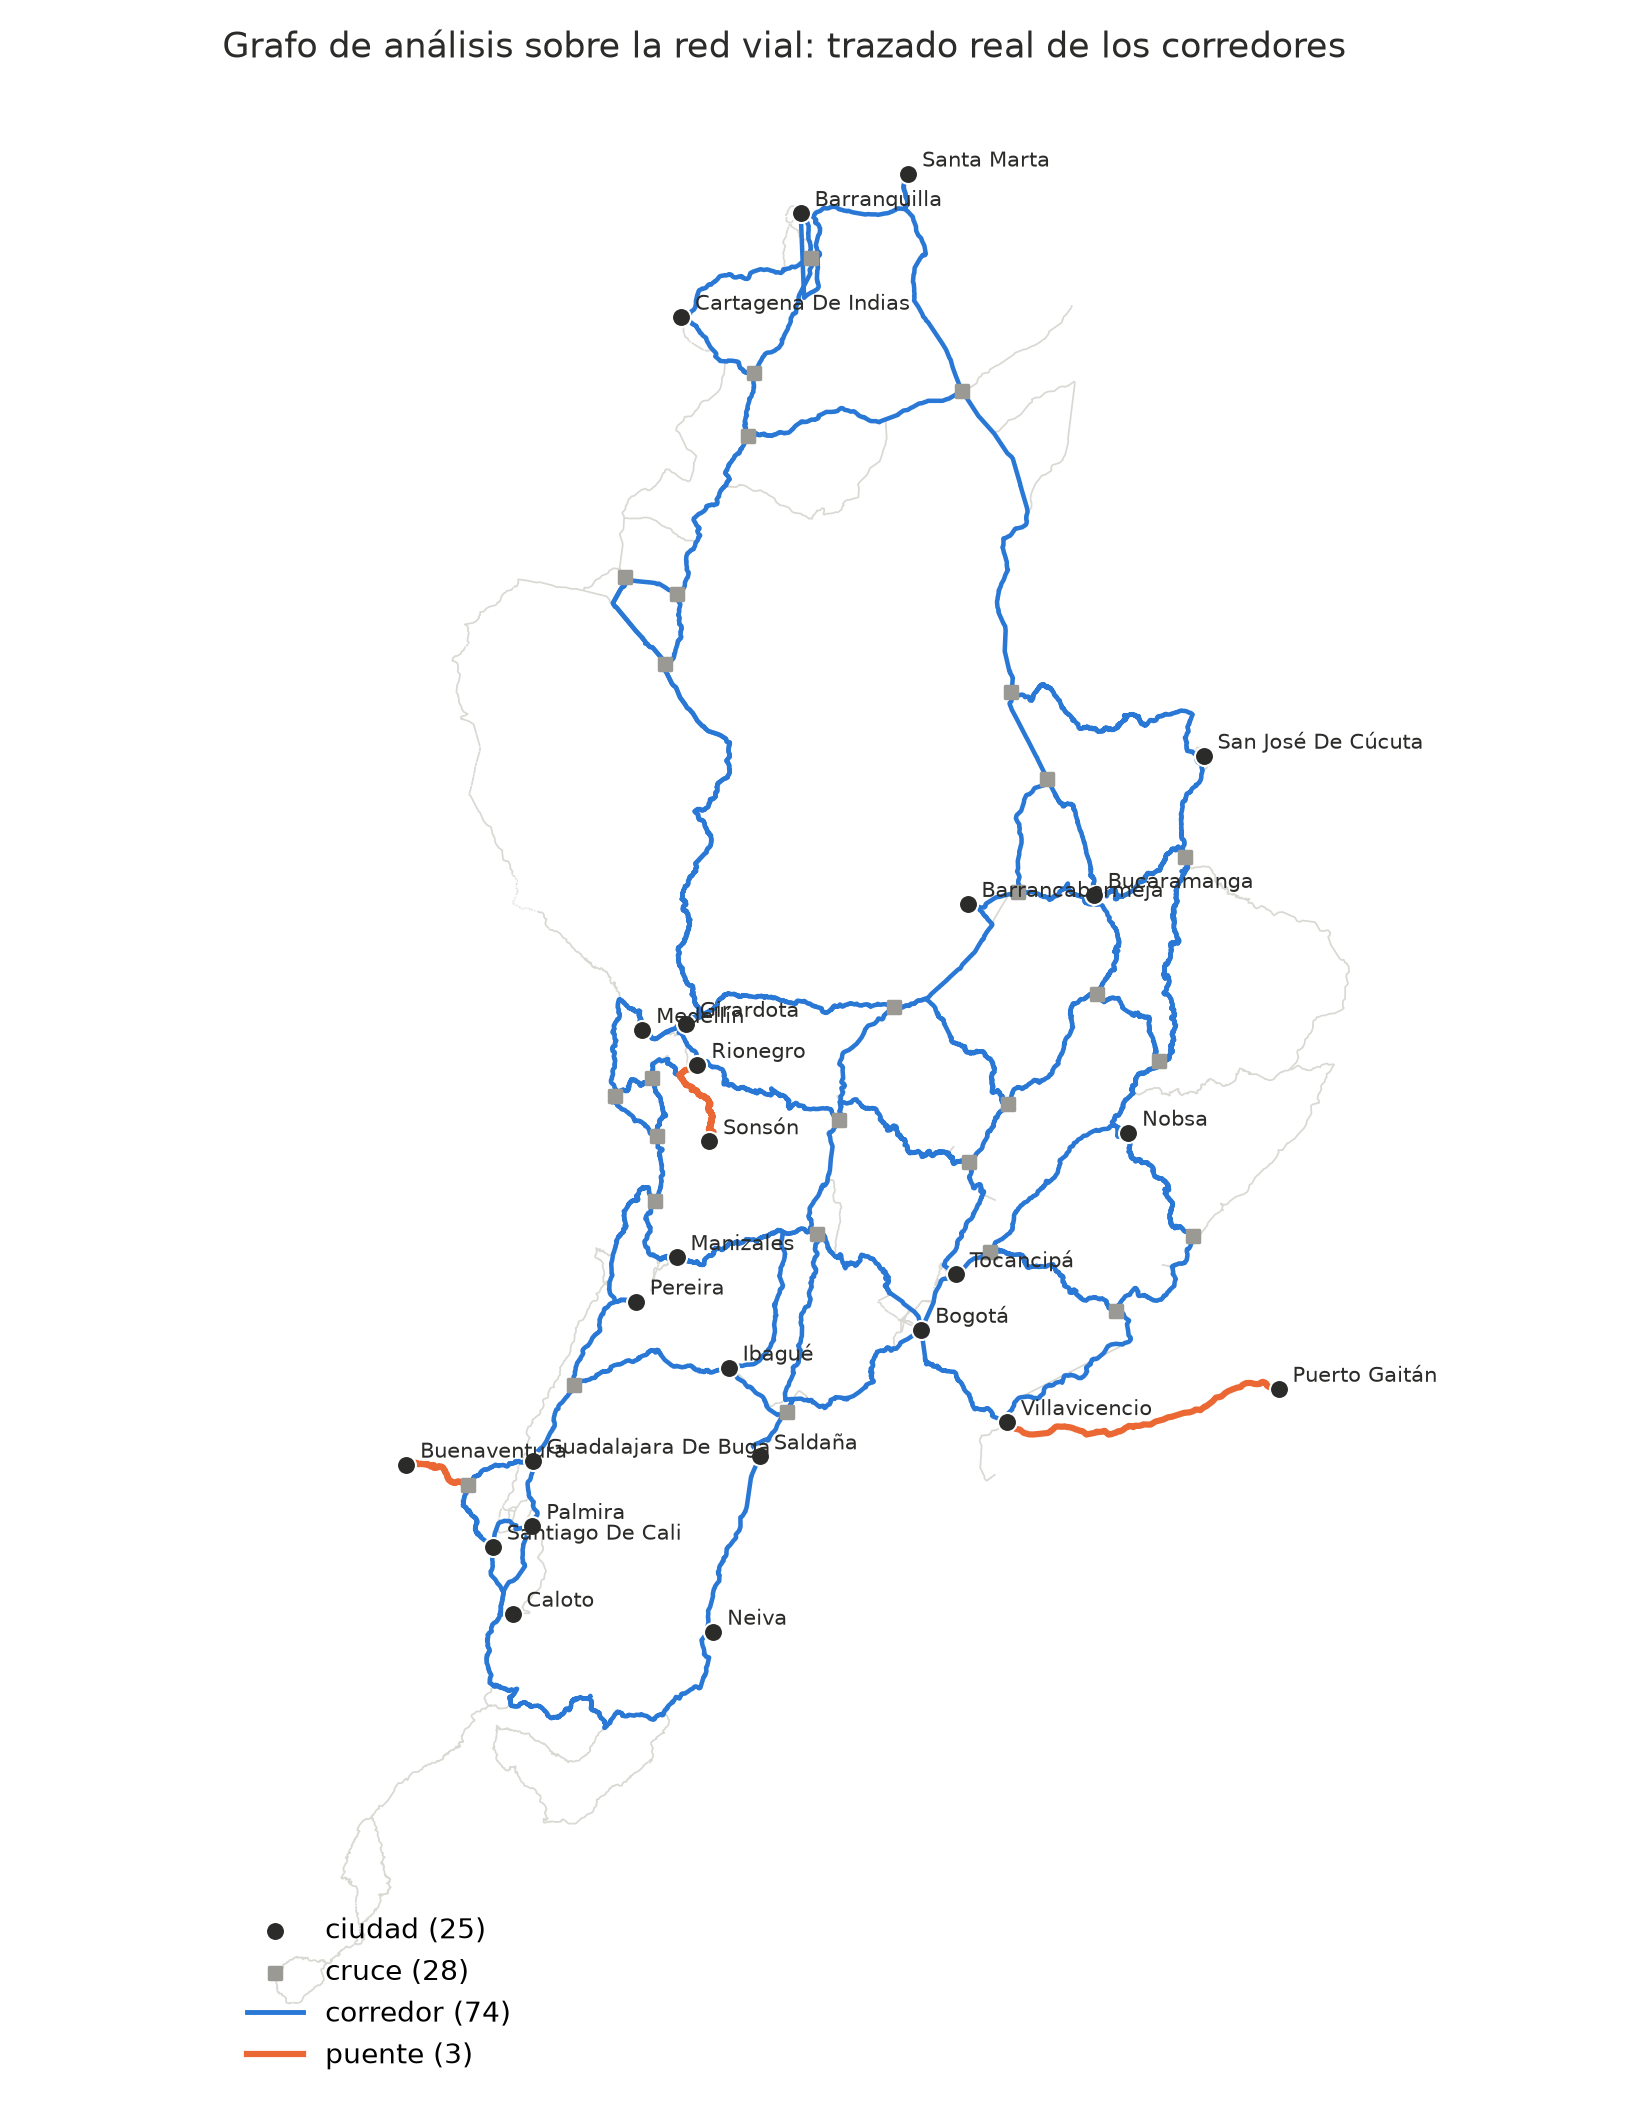
\includegraphics[width=\columnwidth,height=0.45\textheight,keepaspectratio]{grafo_analisis_mapa.png}
    \caption{Grafo de análisis sobre el mapa de Colombia: 25 ciudades, 28
    cruces y 77 corredores. En naranja, los puentes: Buenaventura--Dagua,
    Villavicencio--Puerto Gaitán y Rionegro--Sonsón.}
    \label{fig:mapa}
\end{figure}

\subsection{Cierres y supuestos}
Cerrar una vía equivale a retirar del grafo la arista $e$, o el conjunto de
aristas $S$ que recorre un tramo de INVIAS, y medir el daño con $I$ y $D$. El
modelo supone que la carga no cambia ante un cierre, que no hay congestión (por
lo que el sobrecosto calculado es un mínimo) y que el flete es igual en toda la
red, de modo que las rutas más baratas coinciden con las más cortas.

% ------------------------------------------------
% VI. Solución Propuesta
% ------------------------------------------------
\section{Solución Propuesta}
\label{sec:solucion}

La propuesta es mirar cada tramo desde tres ángulos: su \emph{posición} en la
red (intermediación), su \emph{uso} (la carga que lo atraviesa) y la
\emph{consecuencia de perderlo} (el sobrecosto y la carga sin ruta si se
cierra). Si los tres coincidieran, bastaría con mirar el mapa para saber qué
vías proteger; la hipótesis del proyecto es que no coinciden, y que en esas
diferencias están los tramos cuya importancia se subestima.

El primer ángulo depende solo del grafo. Los otros dos dependen de la matriz
$T$, y por eso es ella la que da el contenido económico al análisis. El proceso
es el siguiente. Primero se describe la red y se identifican sus puentes con
Tarjan. Luego se calcula la situación normal: con Dijkstra se obtienen las
rutas más baratas entre ciudades y sobre ellas se reparte la carga de $T$. Con
eso se comparan la intermediación y la carga de cada arista. Por último se
cierra, una por una, cada arista y cada tramo de INVIAS, y se mide el daño con
el Algoritmo~\ref{alg:cierres}.

\begin{algorithm}[t]
\caption{Simulación del cierre de un conjunto de aristas $S$}
\label{alg:cierres}
\begin{algorithmic}[1]
\Require $G$, $T$, costos sin cierre $c_G(o,d)$, aristas cerradas $S$
\Ensure sobrecosto $I$ y demanda insatisfecha $D$
\State $G' \gets G - S$; \ $I \gets 0$; \ $D \gets 0$
\ForAll{ciudad de origen $o$}
    \State calcular $c_{G'}(o,d)$ para todo $d$ con Dijkstra
    \ForAll{ciudad de destino $d$ con $T_{od}>0$}
        \If{$c_{G'}(o,d)=\infty$}
            \State $D \gets D + T_{od}$ \Comment{sin ruta}
        \Else
            \State $I \gets I + T_{od}\,[\,c_{G'}(o,d)-c_G(o,d)\,]$
        \EndIf
    \EndFor
\EndFor
\State \Return $I$, $D$
\end{algorithmic}
\end{algorithm}

Los resultados se leerán en términos económicos. Como $T$ es la carga de un
año, $I(e)$ es lo que costaría un cierre de todo un año, y un cierre de $k$
días cuesta aproximadamente $I(e)\,k/365$; así se puede estimar, por ejemplo,
el costo de un derrumbe que bloquee una vía durante dos semanas. Además, cada
tramo se ubicará en uno de cuatro grupos según cuánta carga mueve y qué tan
buena es su alternativa. Los críticos son los que mueven mucha carga y no
tienen una alternativa barata.

% ------------------------------------------------
% VII. Implementación de la Solución
% ------------------------------------------------
\section{Implementación de la Solución}
\label{sec:implementacion}

La solución se implementó en Python~3.11; la depuración del RNDC se hizo en R.
El código, los datos y las instrucciones para reproducir cada cifra están en
un repositorio público \cite{repositorio}. Todos los parámetros del modelo
(tolerancias, radios, tarifa) están en un solo archivo de configuración, y las
versiones de las librerías están fijadas, de modo que dos ejecuciones dan
exactamente los mismos archivos.

\subsection{Flujo de trabajo}
El proceso se divide en pasos que se corren en orden; cada uno lee lo que
produjo el anterior (Tabla~\ref{tab:pasos}). Todo el análisis, desde la capa
de INVIAS hasta las figuras, tarda unos 2,5 minutos en un computador personal.

\begin{table}[t]
\caption{Pasos de la implementación}
\label{tab:pasos}
\centering
\footnotesize
\begin{tabular}{@{}cp{3.1cm}p{3.6cm}@{}}
\toprule
Paso & Qué hace & Resultado \\
\midrule
01 & Depura el RNDC y la DIVIPOLA (R) & matriz O-D de 42.547 parejas \\
02 & Limpia el mapa y conecta 50 ciudades & red detallada $D$: 842 nodos, 972 aristas \\
03 & Ciudades, cruces y corredores & grafo $G$: 53 vértices, 77 aristas \\
04 & Propiedades y validación & puentes, $\kappa$, $\lambda$, km vs.\ RNDC \\
05 & Cierres (Algoritmo~\ref{alg:cierres}) & $I$ y $D$ de 77 aristas y 243 tramos \\
06 & Pruebas con respuestas a mano & 9 de 9 superadas \\
07 & Intermediación y carga & $C_B(e)$, $x_e$ y su comparación \\
08 & Figuras & Figs.~\ref{fig:mapa}--\ref{fig:criticos} \\
\bottomrule
\end{tabular}
\end{table}

\subsection{Del mapa al grafo}
La capa de INVIAS no es un grafo: sus tramos vienen de fuentes distintas, se
cruzan sin un vértice común y sus extremos no siempre coinciden. Al unir sus
extremos sin corregir nada, la red queda partida en 464 componentes. La
limpieza separa cada tramo en sus 6.020 líneas, simplifica la geometría con el
algoritmo de Douglas--Peucker \cite{douglas1973} (tolerancia de 5\,m), elimina
1.341 líneas duplicadas o de segunda calzada, parte las vías en los cruces en
T y en X y une los extremos a menos de 50\,m; con eso quedan 22 componentes. La
red detallada $D$ resultante, con las 50 ciudades conectadas, tiene 842 nodos,
972 aristas y 11.866\,km, y es conexa. Sobre ella se construye $G$ como se
describió en la Sección~\ref{sec:modelo}. Al resumir $D$ en $G$ las rutas entre
ciudades cuestan en promedio un 4,0\,\% más (como máximo un 21,4\,\%).

\subsection{Algoritmos}
\textbf{Dijkstra.} Se programó una versión propia con montículo binario, que
corre en $O((n+m)\log n)$ y devuelve, además de los costos, el vértice previo
de cada uno, con el que se reconstruye la ruta. Se comprobó contra la
implementación de NetworkX \cite{hagberg2008} en 200 parejas de ciudades
escogidas al azar: los costos coinciden en todas.

\textbf{Asignación.} Con un Dijkstra desde cada una de las 25 ciudades se
obtienen todas las rutas más baratas; luego, para cada pareja con carga, se
suman sus toneladas a cada arista de su ruta, según \eqref{eq:flujo}. Si una
pareja tiene dos rutas igual de baratas, la carga va completa por la que
encuentra Dijkstra.

\textbf{Brandes y Tarjan.} La intermediación de aristas se calcula entre las
25 ciudades con el algoritmo de Brandes, y los puentes y vértices de corte con
el de Tarjan, ambos en las versiones de NetworkX \cite{hagberg2008}.

\textbf{Cierres.} El Algoritmo~\ref{alg:cierres} se aplica a cada una de las
77 aristas y a cada uno de los 243 tramos de INVIAS que recorre el grafo. Un
tramo cierra una arista si la recorre al menos 1\,km (o la mitad del tramo, si
este es más corto); así no cuentan los metros que varios corredores comparten
al entrar a una ciudad. Como varios tramos cierran las mismas aristas, hay 100
cierres distintos. Cada cierre exige 25 ejecuciones de Dijkstra sobre 53
vértices, y la simulación completa tarda unos 3 segundos: por eso fue posible
cerrar todas las aristas y todos los tramos, sin muestreo.

\textbf{Clasificación.} Cada arista con carga se ubica en uno de cuatro grupos
según dos preguntas: si su carga $x_e$ está por encima de la mediana y si el
sobrecosto por tonelada desviada, $I(e)/x_e$, está por encima de la mediana.
Los puentes cuentan como ``alternativa mala'', porque no tienen ninguna.

\subsection{Verificación}
Cada cálculo se comprobó en un grafo de juguete de 13 vértices cuyas
respuestas se obtuvieron a mano: costos mínimos, ruta y ausencia de ruta,
puentes, carga asignada y cuatro tipos de cierre (con desvío barato, con desvío
caro, de un puente y de dos aristas a la vez). Por ejemplo, cerrar la arista
$C$--$D$ obliga a una carga de 100\,t a desviarse 50\,km más, y el programa
debe dar $I=5.000$ y $D=0$. Las 9 pruebas se superan. Además, en las 300
parejas con más carga, los km del grafo son 1,041 veces los km reportados en
el RNDC (ponderado por toneladas; mediana 1,028).

\subsection{Herramienta interactiva}
Para explorar escenarios se construyó una ventana en la que el usuario elige
un origen, un destino, una o varias vías cerradas y la duración del cierre. La
herramienta dibuja la ruta normal y la ruta alterna sobre el mapa e informa
los kilómetros adicionales, el sobrecosto por tonelada y, con las toneladas del
RNDC de esa pareja, el sobrecosto anual y el del periodo de cierre. Si no
queda ruta, lo dice. Por ejemplo, con Buga--Zarzal cerrada la carga de
Buenaventura a Bogotá pasa de 470 a 821\,km: 87.106 pesos más por tonelada y
cerca de 200 mil millones de pesos al año para esa sola pareja.

% ------------------------------------------------
% VIII. Resultados
% ------------------------------------------------
\section{Resultados}
\label{sec:resultados}

\subsection{Estructura de la red}
La Tabla~\ref{tab:estructura} resume las propiedades de $G$. La red es conexa y
planar, pero muy poco redundante: $\kappa(G)=\lambda(G)=1$, de modo que basta
cerrar una sola arista, o perder un solo vértice, para partirla. Hay tres
puentes. El más importante es Buenaventura--Dagua, la única conexión del
principal puerto del Pacífico con el resto de la red; los otros dos son los
únicos accesos de Puerto Gaitán, en los Llanos, y de Sonsón. Los vértices de corte son los
extremos interiores de esos puentes: Dagua, Villavicencio y Rionegro.

\begin{table}[t]
\caption{Propiedades del grafo de análisis $G$}
\label{tab:estructura}
\centering
\footnotesize
\begin{tabular}{@{}lr@{}}
\toprule
Propiedad & Valor \\
\midrule
Vértices (ciudades + cruces) & 53 (25 + 28) \\
Aristas & 77 \\
Grado medio / mínimo / máximo & 2,91 / 1 / 5 \\
Conexo, planar & sí, sí \\
Diámetro (en aristas) & 14 \\
Conectividad $\kappa(G)$, $\lambda(G)$ & 1, 1 \\
Puentes & 3 \\
Vértices de corte & 3 \\
km del grafo / km del RNDC (300 parejas) & 1,041 \\
\bottomrule
\end{tabular}
\end{table}

\subsection{Posición frente a uso}
La intermediación y la carga asignada están correlacionadas (Spearman
$\rho=0{,}76$, Fig.~\ref{fig:dispersion}), pero no ordenan igual las aristas.
Buga--Zarzal es la primera por intermediación (la usa el 32\,\% de las parejas
de ciudades) y la segunda por carga. En cambio, Buenaventura--Dagua es apenas la
28 por intermediación y la tercera por carga: por ella pasa el 21,6\,\% de toda
la carga entre las 25 ciudades, y el mapa la subestima porque solo conecta una
ciudad. Medellín--Girardota pasa del puesto 44 al 14. En el sentido contrario,
Barrancabermeja--Puerto Berrío es la sexta por intermediación (17,7\,\% de las
parejas) pero la 42 por carga: muchas rutas posibles pasan por ella, pero poca
carga real.

\begin{figure}[t]
    \centering
    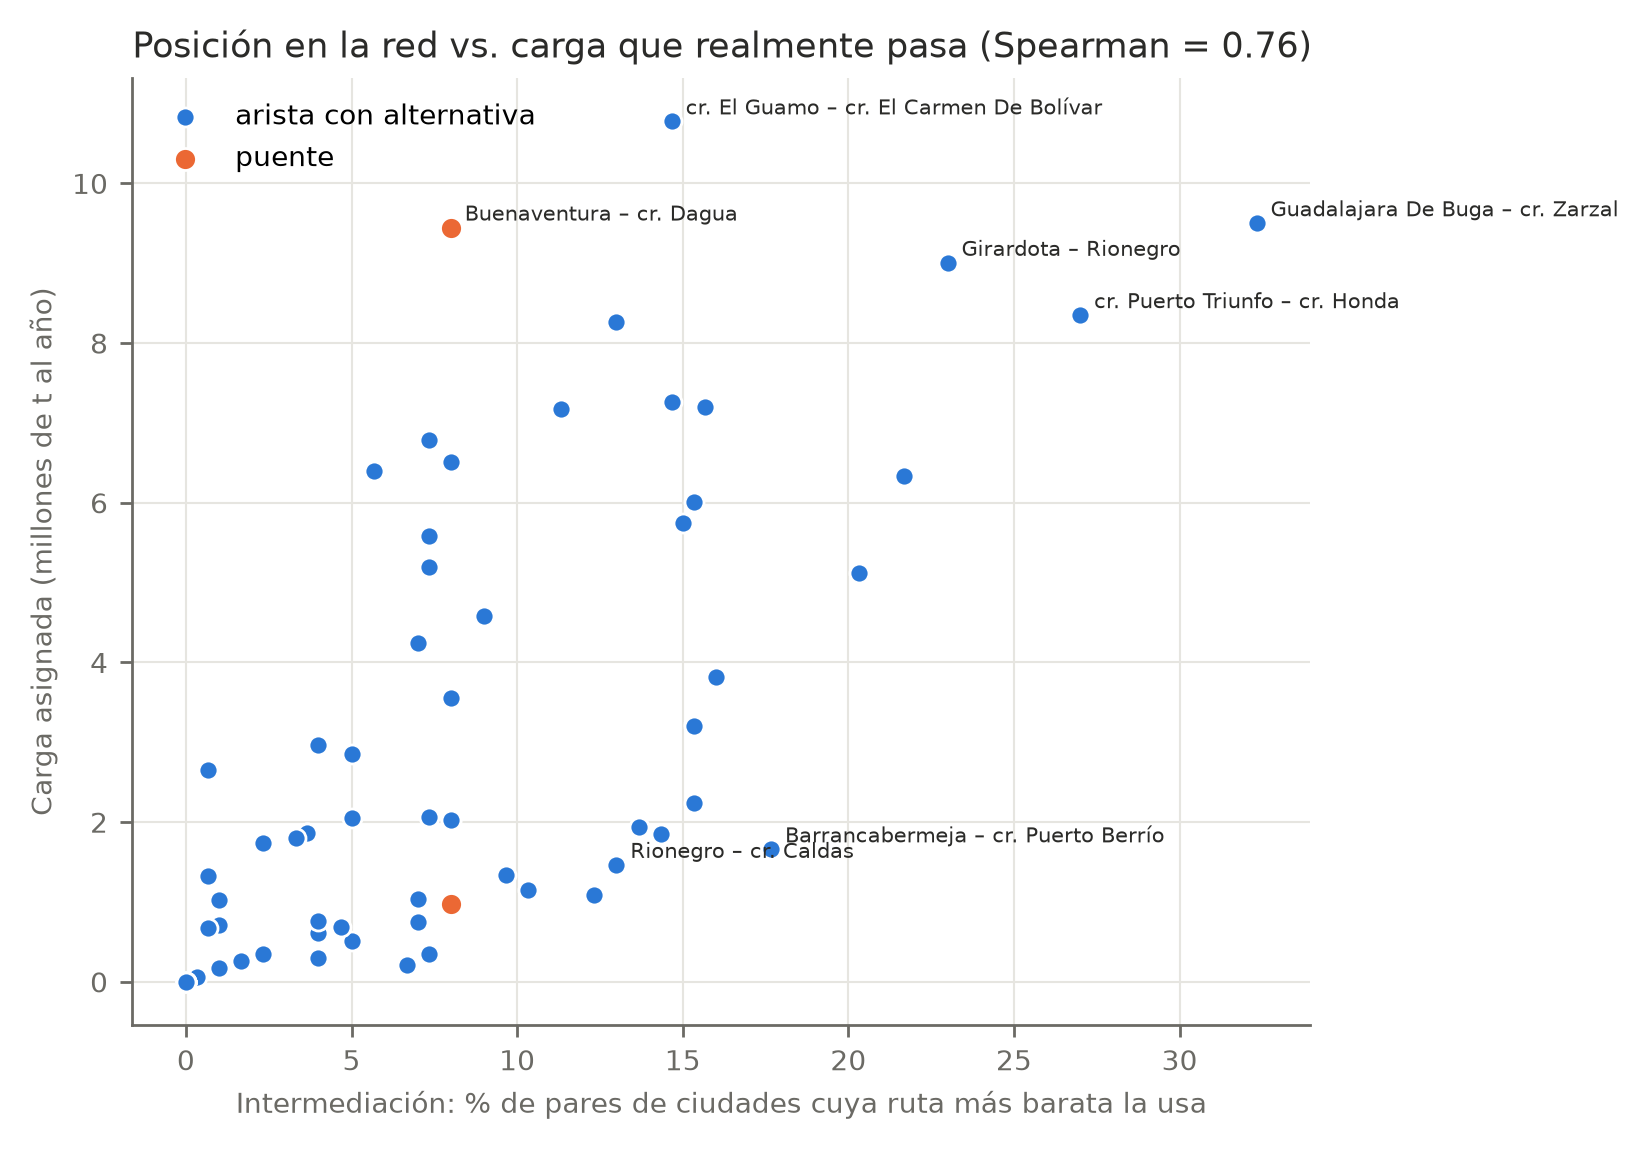
\includegraphics[width=0.92\columnwidth]{carga_vs_intermediacion.png}
    \caption{Intermediación (porcentaje de parejas de ciudades cuya ruta más
    barata usa la arista) frente a la carga asignada. En naranja, los puentes.}
    \label{fig:dispersion}
\end{figure}

\subsection{Consecuencia de los cierres}
\textbf{Carga sin ruta.} Cerrar Buenaventura--Dagua deja sin ruta 9,45
millones de toneladas al año; Villavicencio--Puerto Gaitán, 0,98 millones, y
Sonsón--Rionegro, 0,97 millones. Al cerrar tramos de INVIAS, 18 de los 243
dejan carga sin ruta aunque ninguna de sus aristas sea un puente por sí sola,
porque cortan a la vez los accesos de una ciudad: el tramo Puente
Aurra--Medellín deja 8,14 millones de toneladas sin ruta;
Barranquilla--Santa Marta, 2,73 millones, y El Zulia--Cúcuta, 2,05 millones.

\textbf{Sobrecosto.} La Tabla~\ref{tab:cierres} muestra las aristas cuyo
cierre cuesta más entre las que tienen ruta alterna. Cerrar Buga--Zarzal un año
costaría 908,6 mil millones de pesos; un derrumbe de dos semanas, 34,8 mil
millones. La carga que se desvía paga 95.630 pesos más por tonelada, porque la
alternativa obliga, por ejemplo, a llevar la carga de Buenaventura a Bogotá por
Cali y Neiva. El sobrecosto por tonelada más alto lo tiene Saldaña--Espinal
(147.095 pesos), aunque mueve poca carga.

\begin{table}[t]
\caption{Aristas con mayor sobrecosto al cerrarse (sin puentes)}
\label{tab:cierres}
\centering
\footnotesize
\begin{tabular}{@{}lrrrr@{}}
\toprule
Arista & $x_e$ & $I(e)$ & 14 días & COP/t \\
 & Mt & \multicolumn{2}{c}{mil M COP} & desviada \\
\midrule
Buga--Zarzal & 9,50 & 908,6 & 34,8 & 95.630 \\
El Guamo--El Carmen & 10,78 & 687,3 & 26,4 & 63.774 \\
Bosconia--Aguachica & 4,58 & 473,0 & 18,1 & 103.329 \\
Ibagué--Zarzal & 6,34 & 383,9 & 14,7 & 60.571 \\
Bogotá--Tocancipá & 5,75 & 327,2 & 12,6 & 56.955 \\
Barranquilla--Palmar & 6,51 & 326,5 & 12,5 & 50.130 \\
El Carmen--Ciénaga de Oro & 8,26 & 282,3 & 10,8 & 34.186 \\
Saldaña--Espinal & 1,85 & 271,9 & 10,4 & 147.095 \\
\bottomrule
\end{tabular}
\end{table}

\subsection{Los tres ángulos}
Sin contar los puentes, el sobrecosto se correlaciona más con la carga
($\rho=0{,}89$) que con la intermediación ($\rho=0{,}79$). Sin embargo, de las
diez primeras aristas por cada medida, solo dos están en las tres listas a la
vez: Buga--Zarzal y Bogotá--Espinal. Puerto Triunfo--Honda es la segunda por
intermediación y la quinta por carga, pero apenas la 20 por sobrecosto, porque
su desvío es barato (13.956 pesos por tonelada); con Girardota--Rionegro pasa
lo mismo (puestos 3, 4 y 17). Bosconia--Aguachica, en cambio, es la 27 por
intermediación y la 21 por carga, pero la tercera por sobrecosto.

La clasificación en cuatro grupos (Figs.~\ref{fig:cuadrantes} y
\ref{fig:criticos}) resume esas diferencias: 18 aristas son críticas (mucha
carga y mala alternativa), 14 son importantes pero tienen respaldo, 17 son
vulnerables locales (poca carga y mala alternativa), 18 son secundarias y 10 no
reciben carga. Las críticas se concentran en tres zonas: el corredor del
Pacífico y el Eje Cafetero hacia Bogotá (Buenaventura--Dagua, Buga--Zarzal,
Ibagué--Zarzal, Pereira--Zarzal), el de la costa Caribe (El Guamo, El Carmen de
Bolívar, Bosconia, Aguachica) y los accesos a Bogotá y Medellín.

\begin{figure}[t]
    \centering
    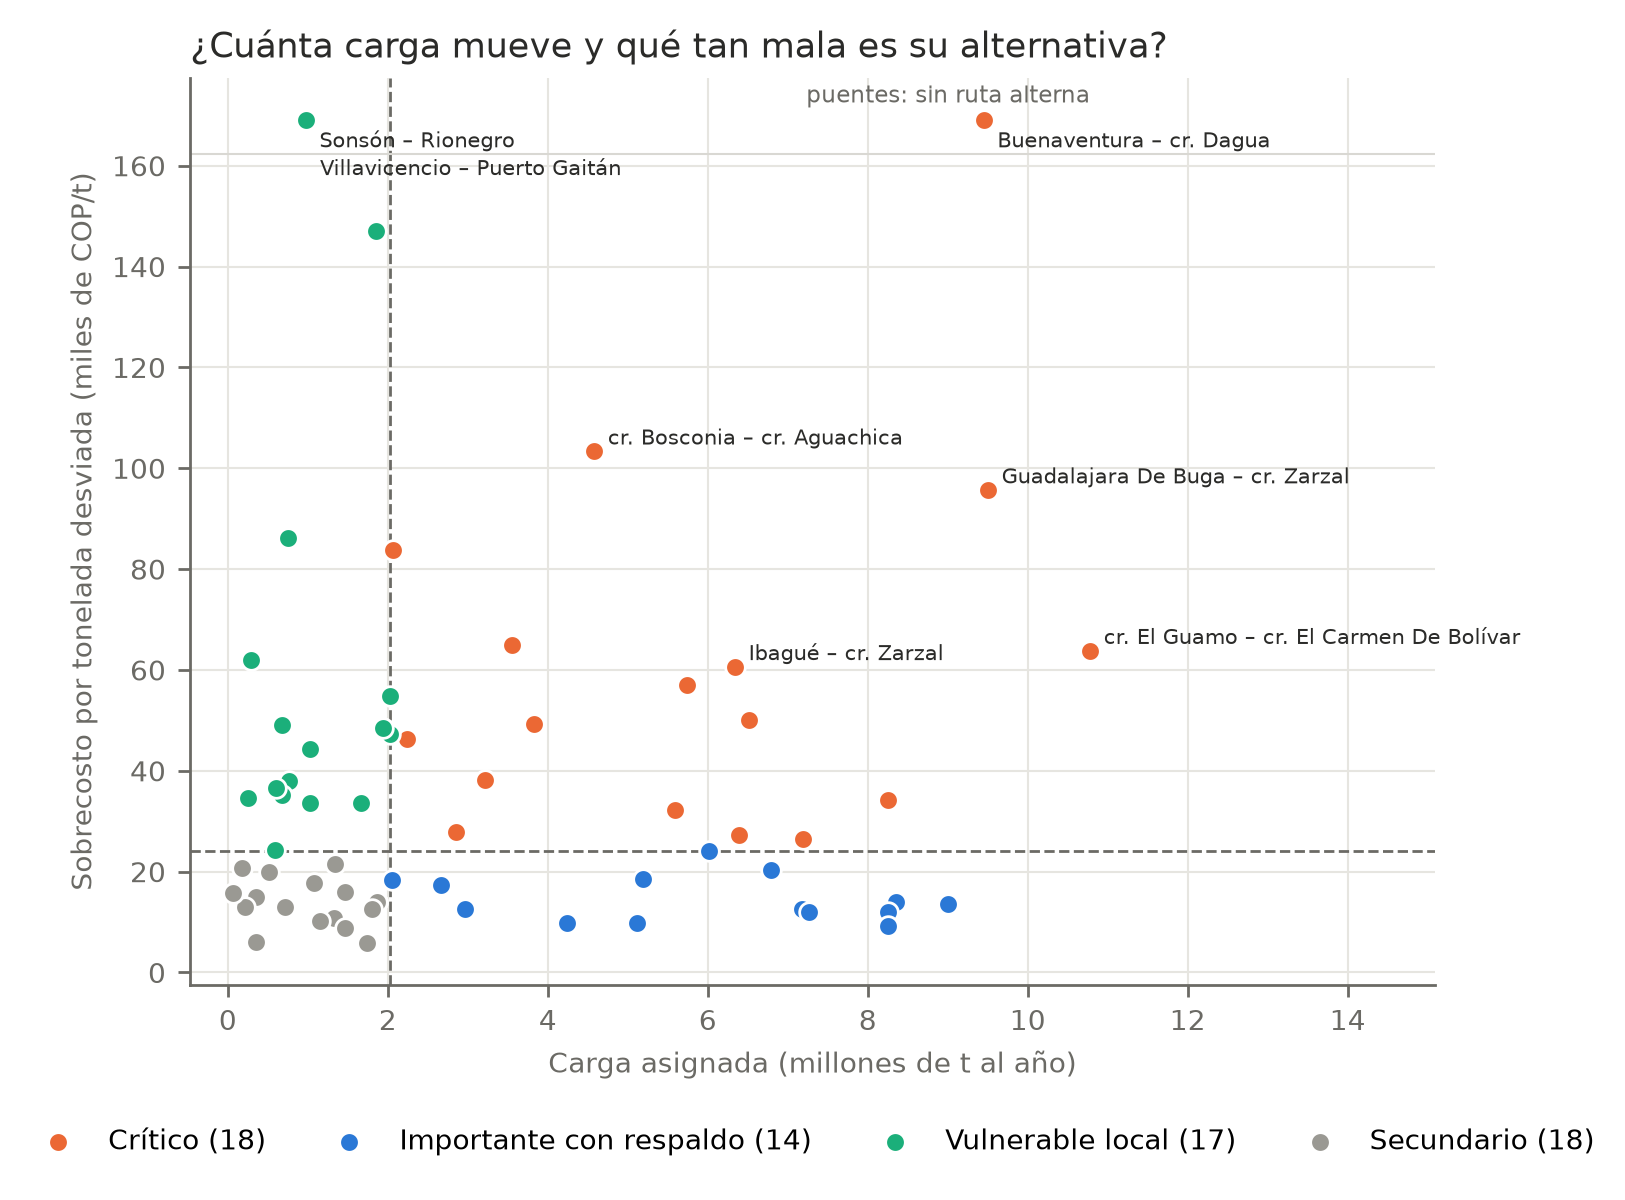
\includegraphics[width=\columnwidth]{cuadrantes.png}
    \caption{Carga asignada frente al sobrecosto por tonelada desviada. Las
    líneas punteadas son las medianas; los puentes van arriba porque no tienen
    alternativa.}
    \label{fig:cuadrantes}
\end{figure}

\begin{figure}[t]
    \centering
    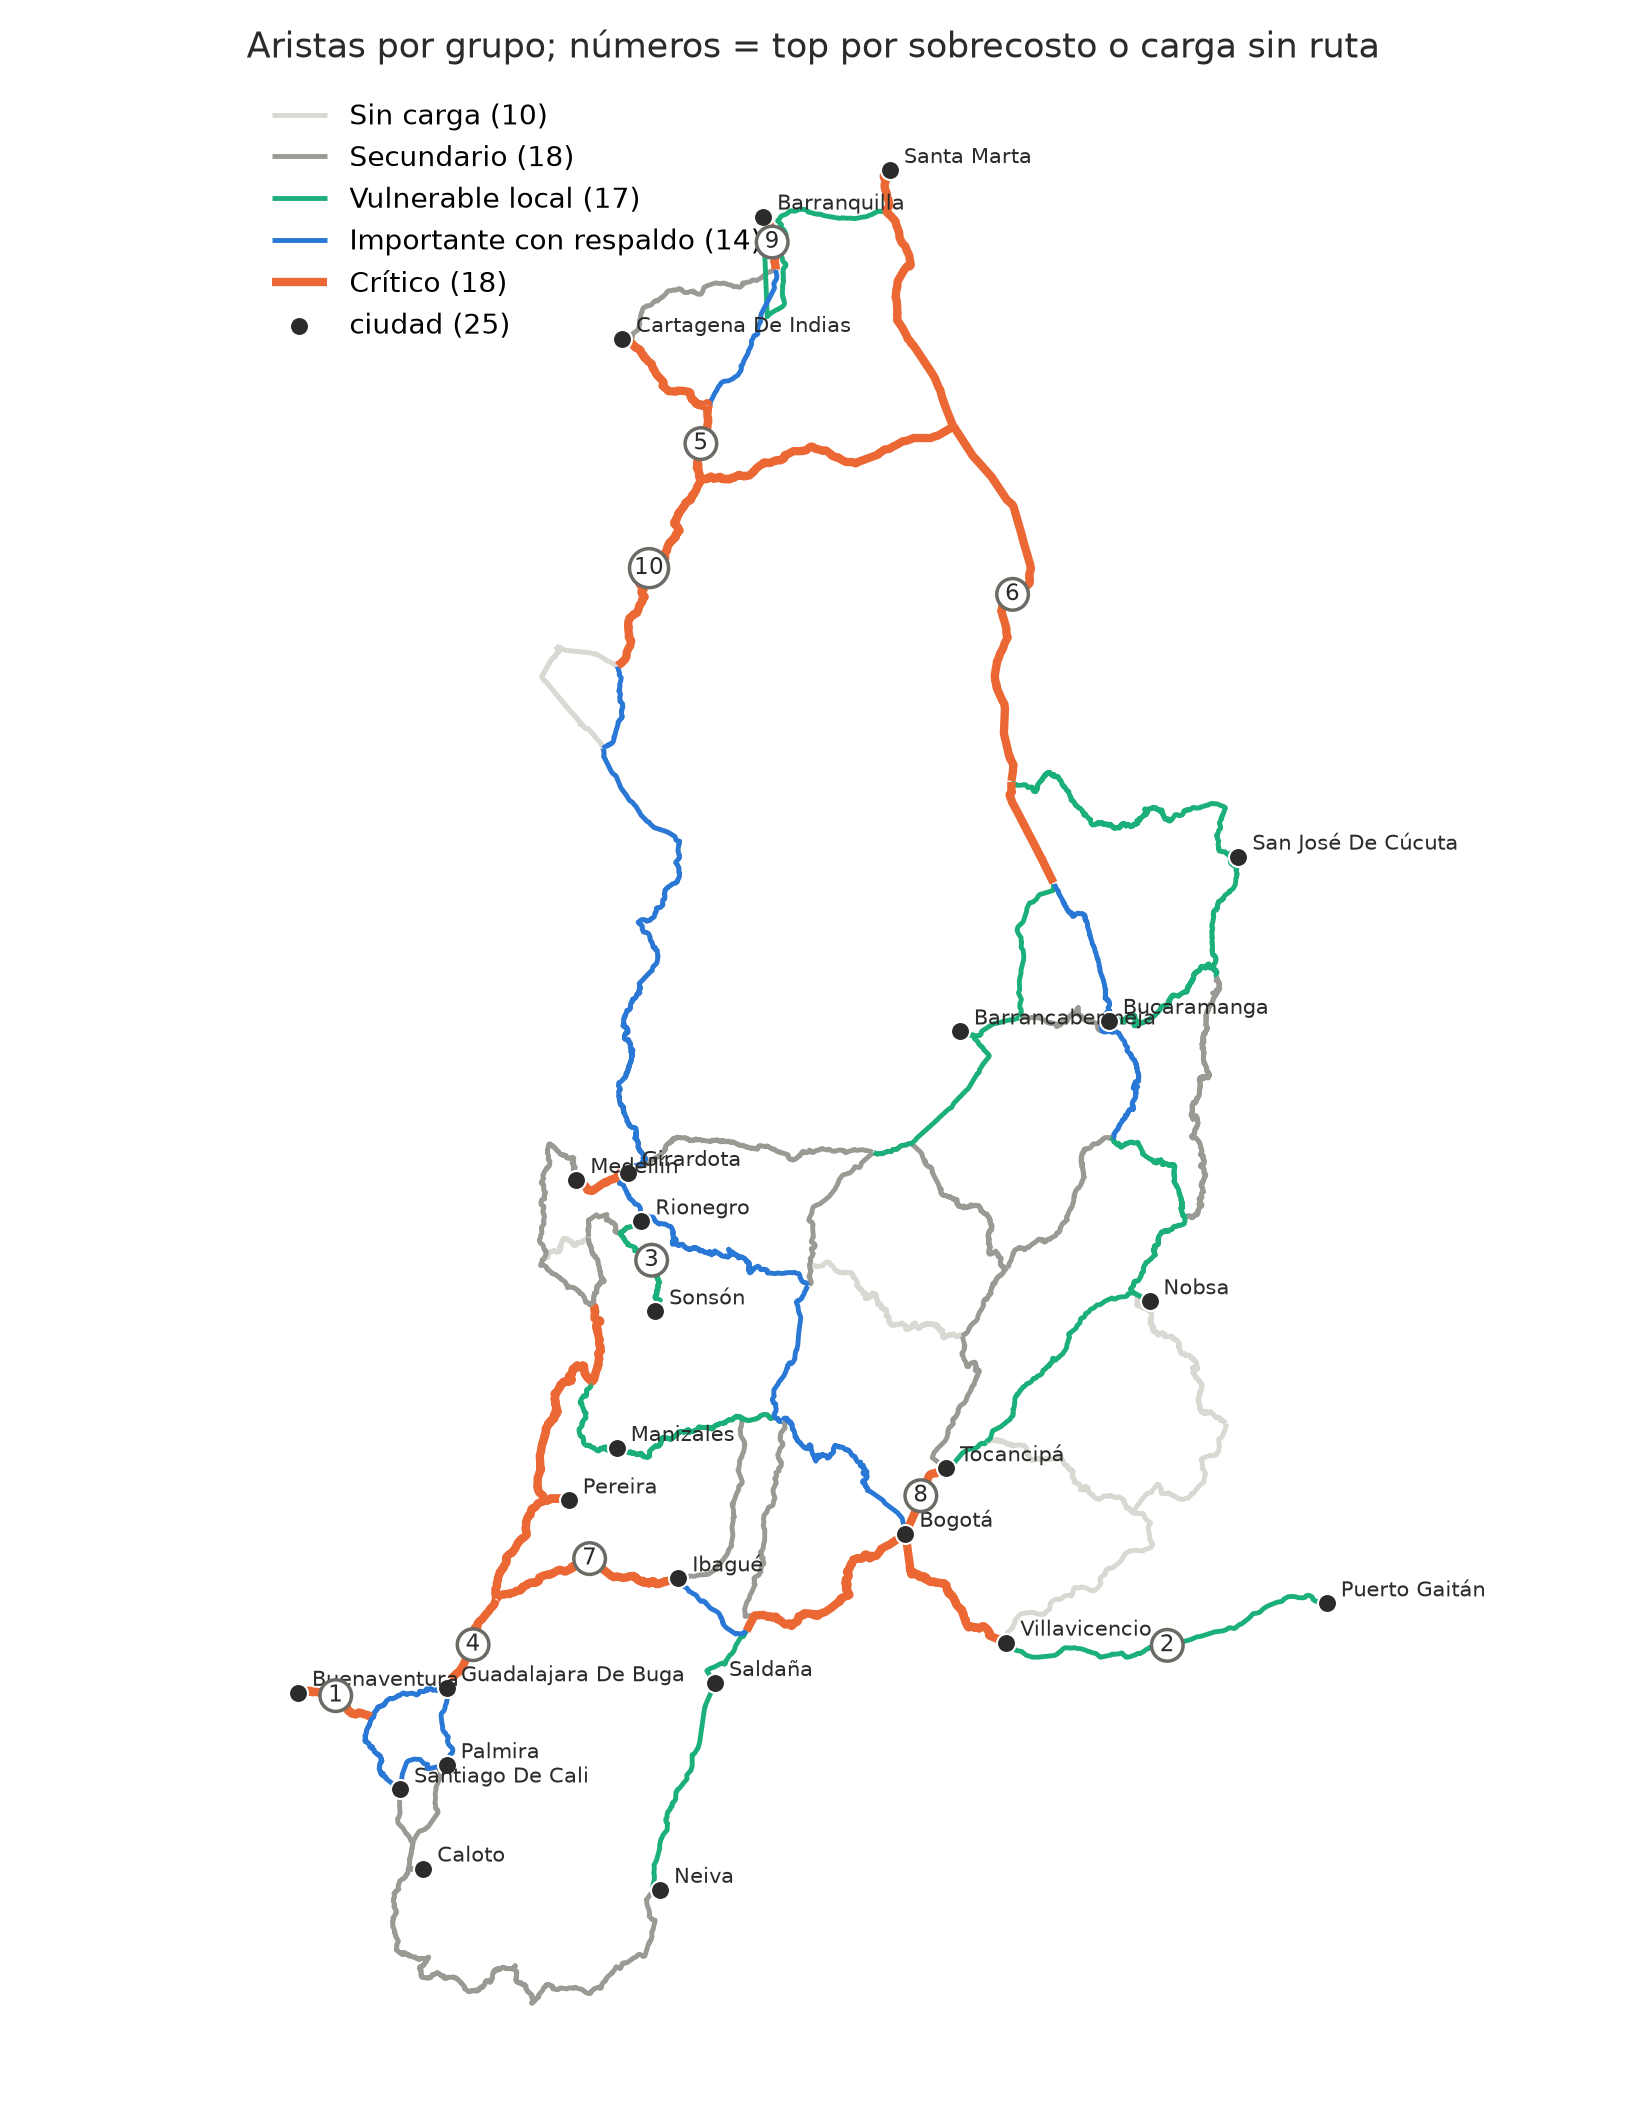
\includegraphics[width=\columnwidth,height=0.42\textheight,keepaspectratio]{mapa_criticos.png}
    \caption{Aristas por grupo. Los números son las diez aristas con mayor
    carga sin ruta o mayor sobrecosto.}
    \label{fig:criticos}
\end{figure}

% ------------------------------------------------
% IX. Conclusiones
% ------------------------------------------------
\section{Conclusiones}
\label{sec:conclusiones}

\textbf{Qué tramos causan más daño.} Con ruta alterna, los cierres más costosos
son Buga--Zarzal (908,6 mil millones de pesos al año), El Guamo--El Carmen de
Bolívar (687,3) y Bosconia--Aguachica (473,0). Sin ruta alterna, el caso más
grave es Buenaventura--Dagua: su cierre deja aislado al principal puerto del
Pacífico y a 9,45 millones de toneladas al año, el 21,6\,\% de la carga entre
las 25 ciudades.

\textbf{La hipótesis se cumple.} Posición, uso y consecuencia están
correlacionados, pero no coinciden: solo dos aristas están entre las diez
primeras de las tres medidas. Mirar solo el mapa sobrestima corredores con
buenas alternativas, como Puerto Triunfo--Honda o Barrancabermeja--Puerto
Berrío, y subestima tramos que mueven mucha carga sin ser pasos obligados para
muchas parejas, como Buenaventura--Dagua o Medellín--Girardota. La carga
predice mejor el daño que la intermediación, pero tampoco basta: lo que hace
crítico a un tramo es la combinación de cuánta carga mueve y qué tan mala es su
alternativa, como se planteó en la Sección~\ref{sec:descripcion}.

\textbf{La red es frágil.} Con $\kappa=\lambda=1$ y tres puentes, una sola falla
puede partirla, y al cerrar tramos completos de INVIAS aparecen más casos sin
ruta, como el acceso a Medellín. Para priorizar el mantenimiento, la inversión
y los planes de contingencia, el grupo de las 18 aristas críticas es una lista
concreta, y la herramienta permite estimar en pesos el costo de un cierre
particular antes de que ocurra.

\textbf{Limitaciones.} El sobrecosto es un mínimo: no hay congestión y la
demanda no cambia ante un cierre. La tarifa es única, así que la ruta más
barata es la más corta. El modelo solo usa la red primaria: algunos desvíos son
largos porque no incluye vías secundarias, y como INVIAS no tiene calles, el
cierre de un acceso urbano puede aislar una ciudad que en la realidad tiene
otra salida. Los datos de carga son de 2015, y solo se simulan cierres de una
arista o de un tramo a la vez.

\textbf{Trabajo futuro.} Usar una tarifa que dependa de cada vía (terreno,
superficie), incluir la red secundaria, simular cierres simultáneos y
ponderarlos por su probabilidad para obtener un costo esperado, asignar la
carga con congestión y actualizar la matriz con datos recientes del RNDC.

% ------------------------------------------------
% Bibliografía
% ------------------------------------------------
\balance
\bibliographystyle{IEEEtran}
\bibliography{references}

\end{document}
